\chapter{Complejos simpliciales}
El espacio topológico asociado a una gráfica con el que trabajaremos, se construye a partir del complejo simplicial de completas de $G$, al cual se le asocia un complejo geométrico que está equipado con una topología. En este capítulo estudiaremos los complejos y la construcción de la realización geométrica de una gráfica.

\section{Complejos simpliciales abstractos}
\label{sec:compl-simpl-abstr}


\begin{Defi}[Complejo simplicial abstracto]
Un complejo simplicial abstracto es una colección $\Delta$ de conjuntos finitos no vacíos tales que si $\sigma$ está en $\Delta$, todo subconjunto no vacío de $\sigma$ también lo está. Un elemento $\sigma$ de $\Delta$ es llamado un simplejo o cara de $\Delta$. 
\end{Defi}

En lo que sigue será frecuente llamar simplemente ``complejo
simplicial'' a un complejo simplicial abstracto.

\begin{Defi}
Sea $\Delta$ un complejo simplicial, $\sigma$ y $\tau$ simplejos de $\Delta$. Definimos los siguientes conceptos:
\begin{enumerate}
\item El conjunto de vértices $V$ de un complejo simplicial $\Delta$ es la unión de sus elementos unipuntuales.
\item Si $\sigma$ contiene $n + 1$ vértices es llamado un $n$-simplejo. La dimensión de $\sigma$ es $n$.
\item Si $\tau\subset\sigma$ decimos que $\tau$ es una cara de $\sigma$. Si la contención es estricta decimos que $\tau$ es una cara propia de $\sigma$.
\item La dimensión de $\Delta$ denotada por $\dim\Delta$ se define
  como $-1$ si $\Delta$ es vacío, como $n$ si $\Delta$ tiene un
  $n$-simplejo, pero no un $(n+1)$-simplejo, o como $\infty$ si $\Delta$ contiene un $n$-simplejo para toda $n\geq 0$.
\end{enumerate}
\end{Defi}
No haremos distinción entre el vértice $v$ que pertenece a $V$ y el 0-simplejo $\{v\}$ que pertenece a $\Delta$.
\begin{Defi}
Una función $f\colon V(\Delta_1)\rightarrow V(\Delta_2)$ es simplicial si para todo simplejo $\sigma$ de $\Delta_1$ se tiene que $f(\sigma)$ es un simplejo en $\Delta_2$.
\end{Defi}
\begin{Defi}
Dos complejos simpliciales $\Delta_1$ y $\Delta_2$ son isomorfos si existe una función biyectiva $f$ de $V(\Delta_1)$ en $V(\Delta_2)$ tal que $f$ es simplicial.
\end{Defi}

\begin{Defi}
Sea $\Delta$ un complejo simplicial, definimos el $p$-esqueleto de $\Delta$ como el complejo simplicial que consiste de todos los simplejos de $\Delta$ de dimensión menor o igual a $p$ y lo denotamos por $\Delta^{(p)}$.
\end{Defi}
%\begin{Ejem}
%Dada una gráfica $G$, denotemos por $\Delta(G)$ la colección de completas de $G$. Es fácil ver que si $c$ es una completa de $G$ entonces cualquier subconjunto no vacío $s$ de $c$ es una completa. Ya que si $x$ y $y$ pertenecen a $s$ entonces $x$ y $y$ pertenecen a $c$ y por lo tanto son adyacentes. En consecuencia $\Delta(G)$ es un complejo simplicial. La dim $\Delta(G)$ es igual al máximo de el conjunto de ordenes de las completas de $G$  y los vértices de $\Delta(G)$ son los vértices de $G$ 
%\end{Ejem}

\section{Complejos simpliciales geométricos}
\subsection{Simplejos en $\mathbb{R}^N$}  
El primer paso para definir un complejo simplicial geométrico, es estudiar las estructuras geométricas que lo conforman, es por ello que la primera parte de esta sección está dedicada a analizar los simplejos en $\mathbb{R}^N$.           
\begin{Defi}[Independencia geométrica]
Dado un conjunto finito $\{a_0,\ldots,a_n\}$ de puntos en $\mathbb{R}^{N}$, el conjunto es geométricamente independiente si la única solución al sistema 
\begin{equation}\label{s1}
    \begin{split}
     &\sum_{i=0}^{n}t_{i} = 0 \\
     &\sum_{i=0}^{n}t_{i}a_{i} = 0   
    \end{split}
\end{equation}

es $t_i = 0$ para toda $i$.
\end{Defi}

Se puede demostrar que un conjunto de puntos es geométricamente
independiente si y solo si no contiene tres puntos colineales, ni
cuatro puntos coplanares, etc.

\begin{Teo}
~\begin{enumerate}[(a)]
    \item El conjunto $\{a_0,\ldots,a_n\}$ es geométricamente independiente si y sólo si $\{a_1-a_0,\cdots,a_n-a_0\}$ es linealmente independiente.
    \item Si $\{a_0,\cdots,a_n\}$ es geométricamente independiente entonces para todo subconjunto no vacío $A$ de $\{a_0,\ldots,a_n\}$, $A$ es geométricamente independiente.
\end{enumerate}
\end{Teo}

\begin{Dem}
\begin{enumerate}[(a)]
\item\label{item:1} Supongamos que $\{a_0,\cdots,a_n\}$ es geométricamente
  independiente. Supongamos una combinación lineal de
  $\{a_1-a_0,\ldots,a_n-a_0\}$ igual a cero, es decir: $\sum_{i=1}^{n}t_i(a_i-a_0)=0$. Reagrupando términos tenemos que: $\sum_{i=1}^{n}t_ia_i + (-\sum_{i=1}^{n}t_i)a_0=0$. Haciendo $t_0 = -\sum_{i=1}^{n}t_i$, se cumple \ref{s1}, al ser $\{a_0,\ldots,a_n\}$ geométricamente independientes se tiene que $t_i=0$ para toda $i$.

Ahora supongamos que el conjunto $\{a_1-a_0,\ldots,a_n-a_0\}$ es linealmente independiente, si $t_0,\ldots,t_n$ son solución del sistema en \ref{s1}, entonces 
\begin{align*}
 0&=\sum_{i=0}^{n}t_ia_i\\
 &=\sum_{i=0}^{n}t_ia_i + (-\sum_{i=0}^{n}t_i)a_0\\
 &=\sum_{i=0}^{n}t_i(a_i-a_0)\\ 
 &= t_0(a_0-a_0) + \sum_{i=1}^{n}t_i(a_i-a_0)\\
 &=\sum_{i=1}^{n}t_i(a_i-a_0)
\end{align*}
Por lo tanto $t_i=0$ para toda $i$.
\item Basta demostrar que al quitarle un elemento al conjunto $\{a_0,\ldots,a_n\}$
el conjunto resultante es geométricamente independiente, sin pérdida
de generalidad consideremos $\{a_0,\ldots,a_n\}\backslash\{a_n\}$. Por~(\ref{item:1}) tenemos que el
conjunto $\{a_1-a_0,\ldots,a_n-a_0\}$ es linealmente independiente, y al quitarle
$a_n-a_0$ sigue siendo linealmente independiente y nuevamente por~(\ref{item:1}) 
tenemos que $\{a_0,\ldots,a_n\}\backslash\{a_n\}$ es geométricamente independiente.
\end{enumerate}
\end{Dem}
Ejemplos:
\begin{enumerate}
\item Conjuntos de un solo punto
\item Todo conjunto linealmente independiente
\item Todo conjunto linealmente independiente unión con el vector cero. 
\end{enumerate}

\begin{Defi}[Simplejo geométrico]
Sea $\{a_0,\ldots,a_n\}$ un conjunto geo\-métricamente independiente en  $\mathbb{R}^{N}$. Definimos el $n$-simplejo geométrico $\sigma$ generado por $a_0,\cdots,a_n$ como el conjunto de todos los puntos $x$ en $\mathbb{R}^{N}$ tales que 
\begin{equation}\label{s2}
\begin{split}
x = \sum_{i=0}^{n}t_ia_i,\\
\sum_{i=0}^{n}t_i=1
\end{split}
\end{equation}
con $t_i\geq 0$ para toda $i$.

Los puntos $a_0,\ldots,a_n$ que generan a $\sigma$ son llamados los
vértices de $\sigma$; y el número $n$ la dimensión de $\sigma$. Cuando
el contexto nos permite distinguir los simplejos geométricos de los
definidos en la sección~\ref{sec:compl-simpl-abstr}, les llamaremos
simplemente ``simplejos''.
\end{Defi}

\begin{figure}[h]
\centering
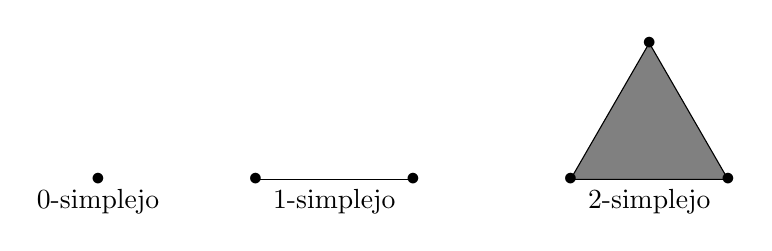
\begin{tikzpicture}
%\draw (-5,-5) grid (5,5);
\draw (-3,0) node {$\bullet$};
\draw (-3,0) node[below] {0-simplejo};

\draw (-1,0)--(1,0);
\draw (0,0) node[below] {1-simplejo};
\draw (-1,0) node {$\bullet$};
\draw (1,0) node {$\bullet$};

\draw [fill = gray] (3,0) -- (5,0) -- (4,1.73205) -- cycle;
\draw (3,0) node {$\bullet$};
\draw (5,0) node {$\bullet$};
\draw (4,1.73205) node {$\bullet$};
\draw (4,0) node[below] {2-simplejo};
\end{tikzpicture}
\caption{Ejemplos de simplejos geométricos}
\end{figure}

Notemos que para $x$ en $\sigma$ los coeficientes $t_i$ están determinados de manera única, ya que si $x = \sum_{i=0}^{n}t_ia_i$ y $x = \sum_{i=0}^{n}s_ia_i$ entonces los $t_i-s_i$ son solución del sistema \ref{s2} por lo que $t_i=s_i$ para toda $i$, lo que nos permite hacer la 
siguiente definición.
\begin{Defi}[Coordenadas baricéntricas]
Sea $\sigma$ un simplejo generado por $a_0,\ldots,a_n$. Si $x$ es un
punto en $\sigma$, entonces $x$ es de la forma $x =
\sum_{i=0}^{n}t_ia_i$ con $t_i\geq 0$, donde los números $t_i$ están
determinados por $x$. Las coordenadas baricéntricas $\{t_i(x):i =
0,\ldots,n\}$ del punto $x$ en $\sigma$ con respecto a $a_0,\ldots,a_n$ se
definen entonces como las funciones de $\sigma\subset\mathbb{R}^N$ en $\mathbb{R}$ tales que $t_i(x) = t_i$.
\end{Defi}

En la siguiente demostración usaremos que una transformación lineal
entre espacios de dimensión finita con la topología inducida por la
norma usual es necesariamente continua. La base canónica de
$\mathbb{R}^N$ se denota como $\{e_1,e_2,\ldots,e_N\}$.

\begin{Prop}
Las coordenadas baricéntricas son continuas.
\end{Prop}
\begin{Dem}

Sea $x$ un punto en $\sigma$, entonces $x=\sum_{i=0}^{n}t_i(x)a_i$ con $\sum_{i=0}^{n}t_i(x)=1$ y 
$t_i(x)\geq 0$, notemos que $t_0(x) = 1-\sum_{i=1}^{n}t_i(x)$ de donde se sigue que:
\begin{equation}
 x = a_0 + \sum_{i=1}^{n}t_i(x)(a_i-a_0)
\end{equation}
El punto $x-a_0$ pertenece al espacio generado por $\{a_1-a_0,\ldots,a_n-a_0\}$ y para $i>0$ las $t_i(x)$  son las coordenadas de $x-a_0$ en la base $\{a_1-a_0,\ldots,a_n-a_0\}$. Si completamos a una base $\{a_1-a_0,\ldots,a_n-a_0,b_{n+1},\ldots,b_N\}$ para $\mathbb{R}^N$,  y definimos la función lineal $T\colon \mathbb{R^N}\rightarrow \mathbb{R^N}$ tal que $T(a_i-a_0) = e_i$ para todo $i=1,\ldots,n$ y $T(b_i) = 0$ para todo $i = n+1,\ldots,N$, tenemos que $T(x-x_0) = (t_1(x),\ldots,t_n(x),0,\ldots,0)$ y como $T$ es continua cada una de sus componentes también lo es, además $t_0(x) = 1-\sum_{i=1}^{n}t_i(x)$ es suma de funciones continuas y por la tanto también es continua. 
\end{Dem}
%Veamos que las coordenadas baricéntricas $t_i(x)$ son continuas, para ello definamos la función $T$ de $\sigma$ en $\mathbb{R}^{N}$ como $T(x) = (t_0(x),\ldots,t_n(x),0,\ldots,0)$.
%\begin{Prop}
%T es continua.
%\end{Prop}
%\begin{Dem}
%
%Sea $x$ un punto en $\sigma$, entonces $x=\sum_{i=0}^{n}t_i(x)a_i$ con $\sum_{i=0}^{n}t_i(x)=1$ y 
%$t_i(x)\geq 0$, notemos que $t_0(x) = 1-\sum_{i=1}^{n}t_i(x)$ de donde se sigue que 
%\begin{equation}
%x = a_0 + \sum_{i=1}^{n}t_i(x)(a_i-a_0)
%\end{equation}
%El punto $x-a_0$ pertenece al espacio generado por $\{a_1-a_0,\ldots,a_n-a_0\}$y para $i>0$ las $t_i(x)$  son las coordendas de $x-a_0$ en la base $a_1-a_0,\ldots,a_n-a_0$ por lo tanto son continuas y  como $t_0(x) = 1-\sum_{i=1}^{n}t_i(x)$ también es continua de donde se sigue la continuidad de T. 
%\end{Dem}
Otras definiciones importantes sobre simplejos geométricos se enuncian a continuación:
\begin{Defi}[Caras de un simplejo]
Si $\sigma$ es el simplejo generado por $a_0,a_1,\ldots,a_n$ y $\tau$
es un simplejo generado por algún subconjunto no vacío de $a_0,a_1,\ldots,a_n$, decimos de $\tau$ es una cara de $\sigma$. Si $\tau$ está contenido estrictamente en $\sigma$ decimos que es una cara propia. 
\end{Defi}
\begin{Defi}[Frontera e interior de un simplejo]
Sea $\sigma$ un simplejo, la frontera de $\sigma$ se define como la unión de todas sus caras propias y se denota por $\bd\sigma$. El interior de $\sigma$ se define como  $\interior \sigma = \sigma-\bd\sigma$. 
\end{Defi}
\begin{Prop}
Para un simplejo geométrico $\sigma$ generado por los puntos $a_0,\ldots,a_n$ en $\mathbb{R}^{N}$ se cumplen las siguientes propiedades:
\begin{enumerate}[(a)]
%\item $\sigma$ es igual a la unión de todos los segmentos que unen a $a_0$ con los puntos del simplejo $S$ generado por $a_1,\ldots,a_n$.
\item $\sigma$ es un conjunto convexo y compacto en $\mathbb{R^{N}}$, el cual es igual a la intersección de todos los conjuntos convexos en $\mathbb{R^{N}}$ que contienen a $a_0,\ldots,a_n$.
\item Si $N = n$, entonces $\interior \sigma$ es abierto en $\mathbb{R}^N$ y $\bd \sigma$ es su frontera en  $\mathbb{R}^N$.
\item Dado un simplejo $\sigma$ existe un único conjunto geométricamente independiente que lo genera.
\end{enumerate}
\end{Prop}
\begin{Dem}
\begin{enumerate}[(a)]
\item Sea $x$ y $y$ puntos en $\sigma$, entonces son de la forma
\begin{align*}
&x = t_0(x)a_0+\cdot +t_n(x)a_n ,\\
&x = t_0(y)a_0+\cdot +t_n(y)a_n
\end{align*}
Ahora consideremos las combinaciones convexas de $x$ y $y$. Dadas por 
$\lambda x + (1-\lambda)y$, con $\lambda$ en el intervalo $[0,1]$. 
Reordenando términos tenemos que
$\lambda x + (1-\lambda)y = [\lambda t_0(x)+(1-\lambda)t_0(y)]a_0+\cdots + [\lambda t_n(x)+(1-\lambda)t_n(y)]a_n$. 

Tenemos que $\lambda t_i(x)+(1-\lambda)t_i(y)$ es mayor que cero para toda $i = 0,\ldots ,n$ y además
\begin{align*}
\lambda t_i(x)+(1-\lambda)t_i(y)&=  \sum_{i=0}^{n}\lambda t_i(x)+\sum_{i=0}^{n}(1-\lambda)t_i(y) \\
&= \lambda\sum_{i=0}^{n}t_i(x)+(1-\lambda)\sum_{i=0}^{n}t_i(y)\\ 
&= \lambda + (1-\lambda)\\
& = 1
\end{align*}
Por lo tanto $\lambda x + (1-\lambda)y$ pertenece a $\sigma$.

\item Sea $x$ un punto en $\interior \sigma$, entonces $x$ es de la forma $x = \sum_{i=0}^{n} t_i(x)a_i$, como $x$ no pertenece a ninguna cara propia de $\sigma$ se tiene que $t_i>0$ para toda $i$.
Si extendemos las coordenadas baricéntricas a $R^n$, dando el valor de cero a los puntos en $\mathbb{R}^n-\sigma$, se sigue que las extensiones son continuas en $\mathbb{R}^n$.
Como los puntos en $\interior \sigma$ cumplen que sus coordenadas baricéntricas son estrictamente mayores que cero, se cumple que $\interior \sigma$ es la intersección de las imágenes inversas de las coordenadas baricéntricas sobre el intervalo abierto $(0,1)$, es decir $\interior \sigma = t_i^{-1}((0,1))\cap\cdots\cap t_n^{-1}((0,1))$. Por lo tanto $interior \sigma$ es abierto en $\mathbb{R}^n$. 

Por último como $\sigma$ es cerrado, se tiene que $\bd \sigma = \sigma -\interior \sigma = \bar{\sigma}-\interior \sigma$, de donde se sigue que $\bd \sigma$ es la frontera de $\sigma$ en el sentido usual.
\end{enumerate}
\end{Dem}

\subsection{Complejos en $\mathbb{R}^N$}
\begin{Defi}[Complejo simplicial geométrico]
Un complejo simplicial geométrico $\textit{K}$ en $\mathbb{R}^N$  es una colección de simplejos en $\mathbb{R}^N$ tal que:
\begin{enumerate}
\item Toda cara de un simplejo de $\textit{K}$ está en $\textit{K}$.
\item La intersección de cualesquiera dos simplejos en $\textit{K}$ es una cara de cada uno de ellos.
\end{enumerate} 
\end{Defi}
\begin{Ejem}
Sea $\sigma$ un $n$-simplejo, la colección que consta de $\sigma$ y todas sus caras propias es un complejo simplicial y la denotamos por $\Delta^n$
\end{Ejem} 
\begin{Defi}
Sean $\textit{K}$ y $\textit{L}$ complejos simpliciales geométricos, tales que $\textit{L}$ está contenido en $\textit{K}$, decimos entonces que $\textit{L}$ es un subcomplejo de $\textit{K}$. 
\end{Defi}

\begin{Prop}
Si $\textit{L}$ es una subcolección de un complejo simplicial geométrico $\textit{K}$, tal que contiene todas las caras de sus elementos, entonces $\textit{L}$ es un subcomplejo de $\textit{K}$.
\end{Prop}

\begin{Defi}
El subcomplejo $\textit{L}$ de $\textit{K}$ que contiene a todos los simplejos de $\textit{K}$ de dimensión a lo más p es llamado el p-esqueleto de $\textit{K}$ y se denota por $\textit{K}^{(p)}$. 
El subcomplejo $\textit{K}^{(0)}$ es denominado el conjunto de vértices de $\textit{K}$.
\end{Defi}

\begin{Teo}
Sea $\abs{\textit{K}}$ la unión de los simplejos de $\textit{K}$, si asociamos a cada simplejo de $\textit{K}$ la topología natural como subespacio de $\mathbb{R}^N$, entonces podemos definir una topología para $\abs{\textit{K}}$ declarando  un conjunto $C$ de  $\abs{\textit{K}}$ cerrado si y sólo si para todo simplejo $\sigma$ en  $\textit{K}$, $\sigma\cap C$ es cerrado en $\sigma$.
\end{Teo}
\begin{Dem}

Primero veamos que la intersección  arbitraria de cerrados es cerrada. Supongamos que para toda simplejo $\sigma$, $C_{\alpha}$ cumple que $\sigma\cap C_{\alpha}$ es cerrado en $\sigma$, para toda $\alpha$ en $I\subset \mathbb{R}$.
Sea $C = \cap_{\alpha \in I}C_{\alpha}$, entonces $C\cap\sigma = \cap_{\alpha\in I}(C_{\alpha}\cap\alpha)$, como cada $C_{\alpha}\cap \sigma$ es cerrado en $\sigma$, su intersección también lo es.

Ahora veamos que la unión finita de de cerrados es cerrada. Sean $C_1,\ldots,C_n$ cerrados en $\abs{K}$, entonces para todo $\sigma$ en $K$ tenemos que $C_i \cap \sigma$ es cerrado en $\sigma$ para toda $i =1,\ldots,n$ y como la unión finita de cerrados en $\sigma$ es cerrada tenemos que $\cup C_i\cap\sigma = (\cup C_i)\cap\sigma$ es cerrado en $\sigma$.
\end{Dem}
El espacio $\abs{K}$ es llamado el \textbf{espacio subyacente} de $K$ o el \textbf{politopo} de $K$.

El siguiente teorema nos permite caracterizar las funciones continuas de $\abs{K}$ en algún espacio topológico.
\begin{Teo}\label{ttc}
Una función $f\colon \abs{K}\rightarrow X$ es continua si y sólo si $f|_{\sigma}$ es continua para cada $\sigma$ en $K$
\end{Teo}
\begin{Teo}
Una función $H\colon \abs{K}\times I \to X$ es continua si y solo si $H$ restringida a cada celda $\abs{\sigma}\times I$ es continua.
\end{Teo}
\begin{Teo}
$\abs{K}$ es Hausdorff
\end{Teo}
\begin{Teo}
Si K es finito entonces $\abs{K}$ es compacto.
\end{Teo}
Un ejercicio interesante es comparar la topología definida en $\abs{K}$, con la topología usual como subespacio de $R^{N}$. Notemos que si $B$ es cerrado en $\abs{K}$ con la topología usual, para todo $\sigma$ en $K$, tenemos que $B\cap\sigma$ es cerrado en $\sigma$ y por lo tanto $B$ es cerrado en $\abs{K}$. Por lo tanto la topología usual está contenida en la topología subyacente. Para ver que en general no se da la doble contención consideremos el siguiente ejemplo.
\begin{Ejem}
bsbjsdjhsjd
\end{Ejem}
Como ya vimos las dos topologías son diferentes en general, pero si $K$ es finito no es difícil probar que las dos topologías son la misma, como veremos a continuación.
\begin{Prop}
Sea K un complejo simplicial geométrico finito. Entonces la topología subyacente y la topología usual en $\abs{K}$ son la misma.
\end{Prop}
\begin{Dem}

Primero notemos que $\abs{K}$ es la unión finita de cerrados en $\mathbb{R}^N$ de donde se sigue que $\abs{K}$ es cerrado en $\mathbb{R}^N$. Por lo tanto los cerrados en $\abs{K}$ con la topología usual son cerrados en $\mathbb{R}^N$ que están contenidos en $\abs{K}$.
Supongamos $C$ cerrado en $\abs{K}$, entonces $C\cap\sigma$ es cerrado en $\sigma$ para toda $\sigma$ y como $\sigma$ es cerrado en $\mathbb{R}^N$, $C\cap\sigma$ también lo es. Luego podemos escribir a $C$ como la unión finita de cerrados en  $\mathbb{R}^N$ de la siguiente forma $C=\cup_{\sigma\in K}C\cap\sigma$, de donde se sigue que $C$ es cerrado en $\mathbb{R^N}$.
\end{Dem}
\begin{Defi}[Esquema de vértices]
Sea $K$ un complejo simplicial geométrico, sea $V$ el conjunto de vértices de $K$ y $\mathcal{R}$ la colección de todos los subconjuntos de $V$ tales que generan un simplejo de K. El complejo simplicial $\mathcal{R}$ es llamado el esquema de vértices de $K$.
\end{Defi}

\subsection{Morfismos simpliciales}
\begin{Teo} \label{tms}
Sean $L$ y $K$ complejos simpliciales geométricos y sea $f\colon K^{(0)} \rightarrow \abs{L}$ una función. Supongamos que  para todo simplejo $\sigma$ de $K$, sus vértices $v_0,\ldots,v_n$ cumplen que los puntos $f(v_0),\ldots,f(v_n)$ pertenecen a un simplejo de $L$.
Entonces $f$ puede extenderse a una función continua $g:\abs{K}  \rightarrow \abs{L}$ tal que:
\begin{equation*}
g(x)= \sum_{i=0}^{n}t_i(x)f(v_i), \textrm{ donde }  x= \sum_{i=0}^{n}t_i(x)v_i
\end{equation*}
\end{Teo}
\begin{Dem}

Los puntos $f(v_0),\ldots,f(v_n)$ pertenecen a un simplejo $\tau$ de $L$, como $\tau$ es un conjunto convexo tenemos que $g(x)= \sum_{i=0}^{n}t_i(x)f(v_i)$ es un punto en $\tau$. Así $g$ mapea el simplejo $\sigma$ en un subconjunto del simplejo $\tau$.

Para mostrar la continuidad de $g$ por el teorema \ref{ttc} basta probar que $g$ restringida a $\sigma$ es continua. Sea $\epsilon > 0$ y sean $x$ un punto en $\sigma$, por la continuidad de las coordenadas baricéntricas existen números reales positivos $\delta_{0},\ldots,\delta_{n}$ tales que:
\begin{align*}
&\text{Si }\parallel x-x^{'} \parallel < \delta_{i}\\
&\text{entonces } \abs{t_i(x)-t_i(x^{'})}< \frac{\epsilon}{(n+1)(\parallel f(v_0)\parallel + \ldots+\parallel f(v_n)\parallel})
\end{align*}
Sea $\delta = \min\{\delta_0,\ldots,\delta_n\}$ y $s = \parallel f(v_0)\parallel + \cdots+\parallel f(v_n)\parallel$, si $\parallel x-x^{'}\parallel< \delta$ entonces
\begin{align*}
&\parallel g(x)-g(x^{'})\parallel = \parallel(t_0(x)-t_0(x^{'}))f(v_0)\parallel+\cdots+\parallel(t_n(x)-t_n(x^{'}))f(v_n)\parallel\\
&< \abs{t_0(x)-t_0(x^{'})}\parallel f(v_0)\parallel+\cdots +  \abs{t_n(x)-t_n(x^{'})}\parallel f(v_n)\parallel \\
&< \abs{t_0(x)-t_0(x^{'})}s+\cdots +  \abs{t_n(x)-t_n(x^{'})}s\\
&< \frac{\epsilon}{n+1}+\cdots + \frac{\epsilon}{n+1} = \epsilon
\end{align*}
\end{Dem}
\begin{Defi}
Sean $L$ y $K$ complejos simpliciales geométricos y sea $f\colon K^{(0)} \rightarrow L^{(0)}$ una función. Supongamos que  para todo simplejo $\sigma$ de $K$, sus vértices $v_0,\ldots,v_n$ cumplen que los puntos $f(v_0),\ldots,f(v_n)$ son vértices de un simplejo de $L$. Decimos que la extensión de $f$ dada por el teorema \ref{tms} es el morfismo simplicial lineal inducido por $f$ y lo denotaremos por $\abs{f}$.
\end{Defi}
\begin{Teo}
Suponga $f:K^{(0)}\rightarrow L^{(0)}$ una función biyectiva tal que los vértices $v_0,\ldots,v_n$ de $K$ generan un simplejo si y solo si $f(v_0),\ldots,f(v_n)$ generan un simplejo de $L$. Entonces el morfismo simplicial inducido $\abs{f}\colon \abs{K}\rightarrow\abs{L}$ es un homeomorfismo. Decimos que $\abs{f}$ es un homeomorfismo simplicial.
\end{Teo}

\begin{Col}
\item Existe un homeomorfismo $f$ de el $n$-simplejo $\sigma$ en el disco unitario $D^n$, tal que $\bd \sigma$ es mapeada a $S^{n-1}$, es decir $f(\bd \sigma) = S^{n-1}$.
\end{Col}
\begin{Dem}
Como $\sigma$ está contenido en $\mathbb{R}^N$, para algún $N$, no necesariamente se cumple que $\interior \sigma$ sea abierto en $\mathbb{R}^N$, sin embargo si consideramos el $n$-simplejo $\tau$ en $\mathbb{R}^n$ generado por los vectores canónicos en $R^n$ y el vector cero. Definimos la función $f\colon V(\Delta(\sigma)^n) \to V(\Delta(\tau)^n)$ como $f(a_0) = 0$ y $f(a_i) = e_i$ para $i$ mayor que cero. Entonces $f$ induce un homeomorfismo $\abs{f}$ entre $\sigma$ y $\tau$.
Luego por los  incisos $(a)$ y  $(b)$ de la proposición , $\int \tau$ es un conjunto abierto, convexo y acotado en $\mathbb{R^{n}}$, por el teorema \ref{homeo_esfera} existe un homeomorfismo $g$ entre $\tau$ y $D^n$.
Por el teorema \ref{homeo_esfera} basta probar que 
\end{Dem}

\begin{Defi}
Dos complejos simpliciales geométricos $L$ y $K$ son linealmente isomorfos si existe un homeomorfismo lineal de $K$ en $L$.
\end{Defi}
El teorema principal que nos permite relacionar los complejos simpliciales con los complejos simpliciales geométricos es el siguiente:
\begin{Teo}\label{tpc} 
~\begin{enumerate}
\item Todo complejo simplicial $\Delta$ es isomorfo al esquema de vértices de algún complejo simplicial geométrico $K$.
\item Dos complejos simpliciales geométricos son linealmente isomorfos si y sólo si sus esquemas de vértices son isomorfos como complejos simpliciales.
\end{enumerate}
\end{Teo}

\section{Realización geométrica}
\begin{Defi}
Sea $\Delta$ un complejo simplicial y $K$ un complejo simplicial geométrico tal que el esquema de vértices de $K$ es isomorfo a $\Delta$, decimos que $\abs{K}$ es una realización geométrica de $\Delta$ y la denotamos por $\abs{\Delta}$.
\end{Defi}
Notemos que para un complejo simplicial $\Delta$ pueden existir una infinidad de realizaciones geométricas, sin embargo si $K$ y $K^{'}$ son tales que sus esquemas de vértices son isomorfos a $\Delta$, por el teorema \ref{tpc} $K$ y $K^{'}$ son linealmente isomorfos. De modo que la realización geométrica es única salvo homeomorfismo simplicial.

Como $\Delta$ y el esquema de vértices de $K$ son isomorfos existe una función simplicial biyectiva $f\colon V(\Delta)\rightarrow V(K)$ que mapea a cada vértice $v$ de $\Delta$ en un punto $f(v)$ en $\mathbb{R}^N$ que es un vértice de $K$. Para fines prácticos no haremos distinción entre $v$ y $f(v)$.

\section{Soportes contraíbles}
\begin{Defi}
Suponga $\Delta$ un complejo simplicial y $X$ un espacio. Una función $C$ la cual envía simplejos de $\Delta$ a subespacios de $X$ es un soporte contraíble si:
\begin{enumerate}
\item Para todo simplejo $\sigma$ de $\Delta$, $C(\sigma)$ es contraíble.
\item Si $\tau$ es una cara de $\sigma$, entonces $C(\tau)\subset C(\sigma)$
\end{enumerate}
\end{Defi}
\begin{Defi}
Una función $f\colon \abs{\Delta} \rightarrow X$ está soportada por $C$ si, para cada simplejo $\sigma$ de $\Delta$, $f(\abs{\sigma})\subset C(\sigma)$.
\end{Defi}

\begin{Teo}\label{soportec}
Si $C$ es un soporte contraíble de un complejo simplicial finito $\Delta$ a un espacio $X$, entonces
\begin{enumerate}[(a)]
\item Existe una función continua $g\colon \abs{\Delta}\rightarrow X$ soportada por $C$.
\item Cualesquiera dos funciones continuas soportadas por $C$ son homotópicas.
\end{enumerate}
\end{Teo}
\begin{Dem}
\begin{enumerate}[(a)]
\item Construiremos $g$ por inducción sobre los $n$-esqueletos de $K$. 
Como base de inducción, para cada vértice $v$ en $K^{(0)}$ sea $g(v)$ cualquier punto de $C(v)$.

La hipótesis inductiva es que $g\colon \abs{K^{(n)}} \to X$ es continua y $g(\abs{\sigma})$ está contenida en $C(\sigma)$ para toda $\sigma$ en $K^{(n)}$.

Supongamos que $\tau$ es un $(n+1)$-simplejo, entonces para cada cara
propia de $\sigma$ de $\tau$, sabemos que $g(\abs{\sigma})\subset
C(\sigma)\subset C(\tau)$, por lo tanto $g(\abs{\bd \tau})$ está
contenido en $C(\tau)$. Como $C(\tau)$ es contraíble, por el
teorema~\ref{ext_general}, se obtiene que~$g$ puede ser extendida continuamente a $\abs{\tau}$ de modo que $g(\abs{\tau}) \subset C(\tau)$. 
Como $g$ es continua en cada simplejo se sigue que~$g$ es continua en $\abs{K}$.

\item Supongamos $f$ y $g$ funciones de $\abs{K}$ en $X$, soportadas por $C$. Construiremos por inducción una homotopía $H\colon \abs{K} \to X$ desde $f$ a $g$, es decir con $H(x,0) = f(x)$ y $H(x,1) = g(x)$.
Definamos $H\colon \abs{K}\times\{0,1\} \to X$ por $H(x,0) = f(x)$ y $H(x,1) = g(x)$.
Si $v$ es un vértice de $K$, entonces $f(v)$ y $g(v)$ pertenecen a $C(v)$. Como $C(v)$ es contraíble, $H$ puede extenderse continuamente a $\{v\}\times I$.

La hipótesis de inducción es que $H$ está definida de manera continua en $\abs{K}\times \{0,1\}\cup \abs{K^{(n)}}\times I$ y $H(\abs{\sigma}\times I)$ está contenido en $C(\sigma)$ para cada $\sigma$ en $K^{(n)}$.
Supongamos que $\tau$ es un $(n+1)-$simplejo, entonces para cada cara
propia de $\sigma$ de $\tau$, sabemos que $\abs{\sigma}$ está
contenida en $C(\sigma)$ y que $C(\sigma)$ está contenido en
$C(\tau)$. Por lo tanto
$H(\abs{\bd\tau}\times I)$ está contenida en $C(\tau)$. Se obtiene
entonces que $H$ puede ser extendida continuamente a $\abs{\tau}\times I$ de modo que $H(\abs{\tau}\times I)$ está contenida en $C(\tau)$.
Luego como $H$ es continua en cada celda $\abs{\sigma}\times I$, $H$ es continua en $\abs{K}\times I$.

\end{enumerate}
\end{Dem}

% Local Variables:
% TeX-master: "tesis.tex"
% End:
